\documentclass[11pt,a4paper]{article}
\usepackage[margin=1in]{geometry}
\usepackage{graphicx}
\usepackage{caption}
\usepackage{subcaption}
\usepackage{hyperref}
\usepackage{amsmath,amssymb}
\usepackage{booktabs}
\usepackage{algorithm}
\usepackage{algorithmic}

\title{Exploring Classifier-Free Guidance in Diffusion Models}
\author{Dhruman Gupta, Rushil Gupta \\ Introduction to Machine Learning Final Project}
\date{\today}

\begin{document}
\maketitle

\begin{abstract}
We present an expository study of classifier-free guidance (CFG) in diffusion-based image generation. Leveraging a custom UNet trained on MS COCO captions with a frozen VAE and CLIP text encoder from Stable diffusion v1.4, we explore the qualitative effects of varying CFG weights on sample fidelity and diversity. Results showcase both successful generations on seen prompts and failure modes on novel objects.
\end{abstract}

\section{Introduction and Background}

Generative modeling has witnessed a renaissance with the advent of diffusion-based methods, which achieve remarkable fidelity by simulating a gradual denoising process. In this section, we first review the fundamentals of diffusion models, then discuss how conditioning can steer generation and introduce classifier guidance, and finally describe the more flexible classifier‐free guidance approach that forms the core of our project.

\subsection{Diffusion Models}

Diffusion models \cite{sohl2015deep,ho2020denoising} formulate generation as the reversal of a known, fixed noising process.  Consider a data distribution over images $x_0\sim p_{\mathrm{data}}(x)$, and define a forward Markov chain that progressively adds Gaussian noise:
\begin{equation}\label{eq:forward}
q(x_t \mid x_{t-1}) = \mathcal{N}\!\bigl(x_t;\,\sqrt{1-\beta_t}\,x_{t-1},\,\beta_t I\bigr),\quad t=1,\dots,T,
\end{equation}
where $\{\beta_t\}$ is a small, increasing variance schedule.  After $T$ steps, $x_T$ is essentially isotropic Gaussian noise.

To generate new samples, we learn a parameterized reverse process
\begin{equation}\label{eq:reverse}
p_\theta(x_{t-1}\mid x_t) 
= \mathcal{N}\!\Bigl(x_{t-1};\,\mu_\theta(x_t,t),\,\sigma_t^2 I\Bigr),
\end{equation}
with mean
\[
\mu_\theta(x_t,t)
=\frac{1}{\sqrt{\alpha_t}}\Bigl(x_t-\frac{\beta_t}{\sqrt{1-\bar\alpha_t}}\;\epsilon_\theta(x_t,t)\Bigr),
\]
where $\alpha_t = 1-\beta_t$ and $\bar\alpha_t = \prod_{s=1}^t \alpha_s$.  The network $\epsilon_\theta(x_t,t)$ predicts the noise component at each step.  Training minimizes the denoising objective:
\begin{equation}\label{eq:loss}
\mathcal{L}(\theta)
=\mathbb{E}_{x_0,\epsilon,t}\Bigl[\bigl\|\epsilon-\epsilon_\theta(x_t,t)\bigr\|^2\Bigr],\quad
x_t=\sqrt{\bar\alpha_t}\,x_0+\sqrt{1-\bar\alpha_t}\,\epsilon,\;\epsilon\sim\mathcal{N}(0,I).
\end{equation}
In practice, this simple loss yields stable training and high-quality samples.

\begin{algorithm}[htb]
\caption{Unconditional DDPM Sampling}\label{alg:ddpm}
\begin{algorithmic}[1]
  \STATE \textbf{Input:} noise schedule $\{\beta_t\}_{t=1}^T$, learned model $\epsilon_\theta$
  \STATE $x_T \sim \mathcal{N}(0,I)$
  \FOR{$t=T,\dots,1$}
    \STATE $\hat\epsilon \leftarrow \epsilon_\theta(x_t,t)$
    \STATE $\mu \leftarrow \frac{1}{\sqrt{\alpha_t}}\Bigl(x_t - \tfrac{\beta_t}{\sqrt{1-\bar\alpha_t}}\hat\epsilon\Bigr)$
    \STATE Sample $x_{t-1}\sim \mathcal{N}(x_{t-1};\,\mu,\sigma_t^2 I)$
  \ENDFOR
  \STATE \textbf{return} $x_0$
\end{algorithmic}
\end{algorithm}

\subsection{Conditioning and Classifier Guidance}

While unconditional diffusion can produce diverse samples, many applications demand control over the output, such as generating an image of a specified class or matching a textual prompt $y$.  Ideally, one would sample from the conditional distribution $p(x_0\mid y)$.  Classifier guidance \cite{dhariwal2021diffusion} achieves this by leveraging an auxiliary classifier $p_\phi(y\!\mid\!x_t)$ trained on noisy inputs.  Using Bayes’ rule and score decomposition:
\[
\nabla_{x_t}\log p(x_t\mid y)
=\nabla_{x_t}\log p(x_t)
+\nabla_{x_t}\log p(y\mid x_t),
\]
we adjust the denoising mean in the reverse step:
\begin{equation}\label{eq:clf_guidance}
\tilde{\mu}
=\mu_\theta(x_t,t)
+ s\,\sigma_t^2\,\nabla_{x_t}\log p_\phi(y\mid x_t),
\end{equation}
where $s$ is the guidance strength.  Intuitively, the classifier gradient pushes $x_t$ toward regions where the classifier predicts $y$.

\begin{algorithm}[htb]
\caption{Classifier‐Guided Sampling}\label{alg:clf_guidance}
\begin{algorithmic}[1]
  \STATE \textbf{Input:} schedule $\{\beta_t\}$, model $\epsilon_\theta$, classifier $p_\phi$, strength $s$
  \STATE $x_T \sim \mathcal{N}(0,I)$
  \FOR{$t=T,\dots,1$}
    \STATE $\hat\epsilon \leftarrow \epsilon_\theta(x_t,t)$
    \STATE $\mu \leftarrow \frac{1}{\sqrt{\alpha_t}}\bigl(x_t - \tfrac{\beta_t}{\sqrt{1-\bar\alpha_t}}\hat\epsilon\bigr)$
    \STATE $g \leftarrow \nabla_{x_t}\log p_\phi(y\!\mid\!x_t)$
    \STATE $\mu \leftarrow \mu + s\,\sigma_t^2\,g$
    \STATE Sample $x_{t-1}\sim\mathcal{N}(x_{t-1};\,\mu,\sigma_t^2 I)$
  \ENDFOR
  \STATE \textbf{return} $x_0$
\end{algorithmic}
\end{algorithm}

Although effective, classifier guidance requires training a separate classifier on every noise level and can incur significant compute overhead.  Moreover, classifier gradients may introduce artifacts if the classifier is imperfect.

\subsection{Classifier‐Free Guidance}

Classifier‐free guidance (CFG) \cite{ho2022classifierfree} elegantly sidesteps the need for an external classifier by training the diffusion model itself to operate both with and without conditioning.  During training, each sample’s condition $c$ (e.g.\ text embedding) is randomly dropped with probability $p_\text{drop}$, so the model learns to predict
\[
\epsilon_\theta(x_t,t,c)\quad\text{and}\quad\epsilon_\theta(x_t,t,\varnothing)\,.
\]
At inference, one interpolates between these two predictions:
\begin{equation}\label{eq:cfg}
\epsilon_{\mathrm{CFG}}
=(1+w)\,\epsilon_\theta(x_t,t,c)\;-\;w\,\epsilon_\theta(x_t,t,\varnothing),
\end{equation}
where $w\ge0$ is the guidance weight.  Substituting $\epsilon_{\mathrm{CFG}}$ into the reverse mean (Eq.~\ref{eq:reverse}) yields a sample that balances fidelity to the condition against sample diversity.

\begin{algorithm}[htb]
\caption{Classifier‐Free Guidance Sampling}\label{alg:cfg}
\begin{algorithmic}[1]
  \STATE \textbf{Input:} schedule $\{\beta_t\}$, model $\epsilon_\theta$, weight $w$, condition $c$
  \STATE $x_T \sim \mathcal{N}(0,I)$
  \FOR{$t=T,\dots,1$}
    \STATE $\epsilon_c \leftarrow \epsilon_\theta(x_t,t,c)$
    \STATE $\epsilon_u \leftarrow \epsilon_\theta(x_t,t,\varnothing)$
    \STATE $\epsilon \leftarrow (1+w)\,\epsilon_c - w\,\epsilon_u$
    \STATE $\mu \leftarrow \frac{1}{\sqrt{\alpha_t}}\bigl(x_t - \tfrac{\beta_t}{\sqrt{1-\bar\alpha_t}}\epsilon\bigr)$
    \STATE Sample $x_{t-1}\sim\mathcal{N}(x_{t-1};\,\mu,\sigma_t^2 I)$
  \ENDFOR
  \STATE \textbf{return} $x_0$
\end{algorithmic}
\end{algorithm}

CFG offers several advantages: it requires no extra classifier, allows a single model to flexibly trade off between unconditional and conditional generation, and has been shown to deliver state‐of‐the‐art sample quality with minimal overhead.



\section{Dataset and Preprocessing}
We train on MS COCO 2014 captioned images. Input images are resized and center-cropped to 128×128, then normalized to $[-1,1]$. A custom collate function randomly drops 20\% of captions to implement unconditional conditioning during training.

\section{Model and Training}
\paragraph{Architecture.} We use a frozen VAE and CLIP text encoder from stable-diffusion-v1-4. The UNet is built from scratch with four down/up blocks, two layers each, and cross-attention dimensions matching CLIP (768). An EMA wrapper (decay=0.9999) maintains stable weights.

\paragraph{Training Setup.} Training uses a DDPMScheduler (1,000 timesteps, v\_prediction), AdamW optimizer (lr=1e-4, weight decay=1e-2), CosineAnnealingLR over 450 epochs, batch size=320 with gradient accumulation=4 steps. Training is distributed via \texttt{Accelerate} without mixed precision.

\section{Inference and Sampling}
For sampling, we assemble a \texttt{StableDiffusionPipeline} with DDIMScheduler (1,000 timesteps) and vary guidance weights $w\in\{1.0,3.0,5.0, 7.0\}$. Seed and timesteps are fixed for reproducibility. Grids of 3×3 are generated per prompt and weight.

\section{Results}
We present qualitative grids illustrating the effect of guidance weight. Each subfigure shows nine samples for a given prompt and weight.

\begin{figure}[!ht]
\centering
\begin{subfigure}[b]{0.24\textwidth}
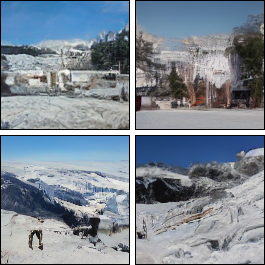
\includegraphics[width=\linewidth]{figures/a_beautiful_snowy_mountain_landscape_1.png}
\caption{$w=1.0$}
\end{subfigure}
\begin{subfigure}[b]{0.24\textwidth}
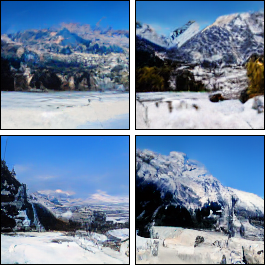
\includegraphics[width=\linewidth]{figures/a_beautiful_snowy_mountain_landscape_3.png}
\caption{$w=3.0$}
\end{subfigure}
\begin{subfigure}[b]{0.24\textwidth}
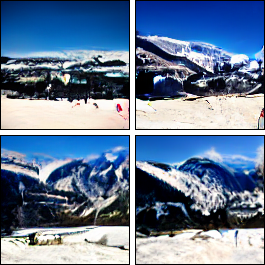
\includegraphics[width=\linewidth]{figures/a_beautiful_snowy_mountain_landscape_5.png}
\caption{$w=5.0$}
\end{subfigure}
\begin{subfigure}[b]{0.24\textwidth}
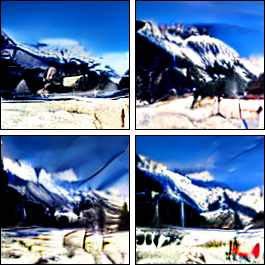
\includegraphics[width=\linewidth]{figures/a_beautiful_snowy_mountain_landscape_7.png}
\caption{$w=7.0$}
\end{subfigure}
\caption{"a beautiful snowy mountain landscape"}
\end{figure}

\begin{figure}[!ht]
    \centering
    \begin{subfigure}[b]{0.24\textwidth}
    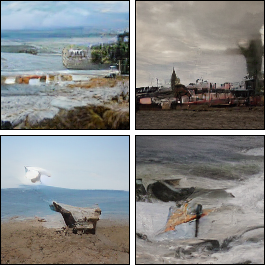
\includegraphics[width=\linewidth]{figures/a_beach_1.png}
    \caption{$w=1.0$}
    \end{subfigure}
    \begin{subfigure}[b]{0.24\textwidth}
    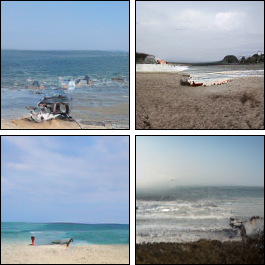
\includegraphics[width=\linewidth]{figures/a_beach_3.png}
    \caption{$w=3.0$}
    \end{subfigure}
    \begin{subfigure}[b]{0.24\textwidth}
    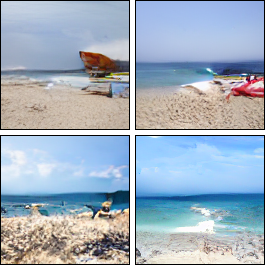
\includegraphics[width=\linewidth]{figures/a_beach_5.png}
    \caption{$w=5.0$}
    \end{subfigure}
    \begin{subfigure}[b]{0.24\textwidth}
    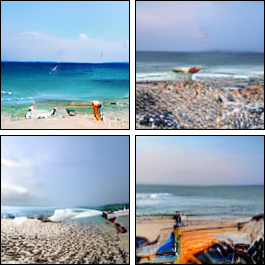
\includegraphics[width=\linewidth]{figures/a_beach_7.png}
    \caption{$w=7.0$}
    \end{subfigure}
    \caption{"a beach"}
    \end{figure}

    \begin{figure}[!ht]
        \centering
        \begin{subfigure}[b]{0.24\textwidth}
        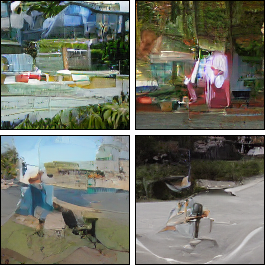
\includegraphics[width=\linewidth]{figures/A_tennis_court_1.png}
        \caption{$w=1.0$}
        \end{subfigure}
        \begin{subfigure}[b]{0.24\textwidth}
        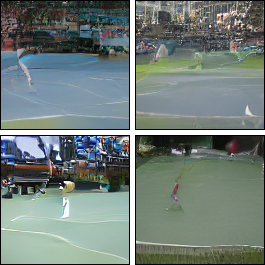
\includegraphics[width=\linewidth]{figures/A_tennis_court_3.png}
        \caption{$w=3.0$}
        \end{subfigure}
        \begin{subfigure}[b]{0.24\textwidth}
        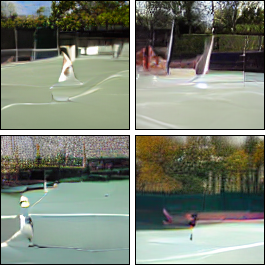
\includegraphics[width=\linewidth]{figures/A_tennis_court_5.png}
        \caption{$w=5.0$}
        \end{subfigure}
        \begin{subfigure}[b]{0.24\textwidth}
        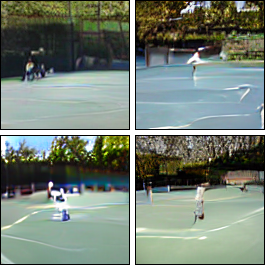
\includegraphics[width=\linewidth]{figures/A_tennis_court_7.png}
        \caption{$w=7.0$}
        \end{subfigure}
        \caption{"a tennis court"}
        \end{figure}

\section{Discussion}
Increasing guidance weight enhances prompt adherence but reduces sample diversity, leading to mode collapse at high $w$. Also, due to our small dataset and limited model parameters, high guidance weights lead to artifacts. Failure cases on novel objects highlight dataset limitations: COCO lacks sufficient examples of uncommon items. The chosen UNet size balances capacity and compute but may underfit complex scenes.

\section{Future Work}
Expanding the training corpus with larger captioned datasets (e.g., OpenImages, LAION) can improve object diversity. Parameter-efficient fine-tuning (LoRA) could enable larger backbone models under compute constraints. Exploring alternative noise schedules and fewer timesteps may accelerate training and improve sharpness.

\section{Conclusion}
We implemented classifier-free guidance in a custom diffusion model and systematically explored its qualitative impact. CFG offers a simple yet powerful control knob for balancing fidelity and diversity. Our findings underscore the importance of dataset scale and model capacity for reliable generative performance.

\bibliographystyle{plain}
\bibliography{refs}

\begin{thebibliography}{4}
    \bibitem{sohl2015deep}
    Sohl-Dickstein, Jascha, Eric A. Weiss, Niru Maheswaranathan, and Surya Ganguli.
    \newblock Deep Unsupervised Learning using Nonequilibrium Thermodynamics.
    \newblock In {\em Proceedings of the 32nd International Conference on Machine Learning (ICML)}, 2015.
    
    \bibitem{ho2020denoising}
    Ho, Jonathan, Ajay Jain, and Pieter Abbeel.
    \newblock Denoising Diffusion Probabilistic Models.
    \newblock In {\em Advances in Neural Information Processing Systems (NeurIPS)}, 2020.
    
    \bibitem{dhariwal2021diffusion}
    Dhariwal, Prafulla and Alex Nichol.
    \newblock Diffusion Models Beat GANs on Image Synthesis.
    \newblock In {\em Advances in Neural Information Processing Systems (NeurIPS)}, 2021.
    
    \bibitem{ho2022classifierfree}
    Ho, Jonathan and Tim Salimans.
    \newblock Classifier-Free Diffusion Guidance.
    \newblock In {\em Advances in Neural Information Processing Systems (NeurIPS)}, 2022.
    \end{thebibliography}
    
    \end{document}